The main objectives of this water treatment device are:

\begin{itemize}

\item{} Obtaining a high degree of purification in the processed water sample, reducing its conductivity by approximately two orders of magnitude (from $1000~\mu$S$/\cm$ up to $10~\mu$S$/\cm$)

\item{} Designing of a device with low maintenance (low cost  and low manpower)

\item{} Installation of a remote control devices such as probes and valves and development of a software to management it.
\end{itemize}

For this, the LARUEX laboratory in Extremadura, one of the six collaborators of the TRITIUM experiment, has designed, developed and built an ultrapure water system, whose scheme is shown in figure \ref{fig:WPSScheme}.

\begin{figure}[htbp]
\centering
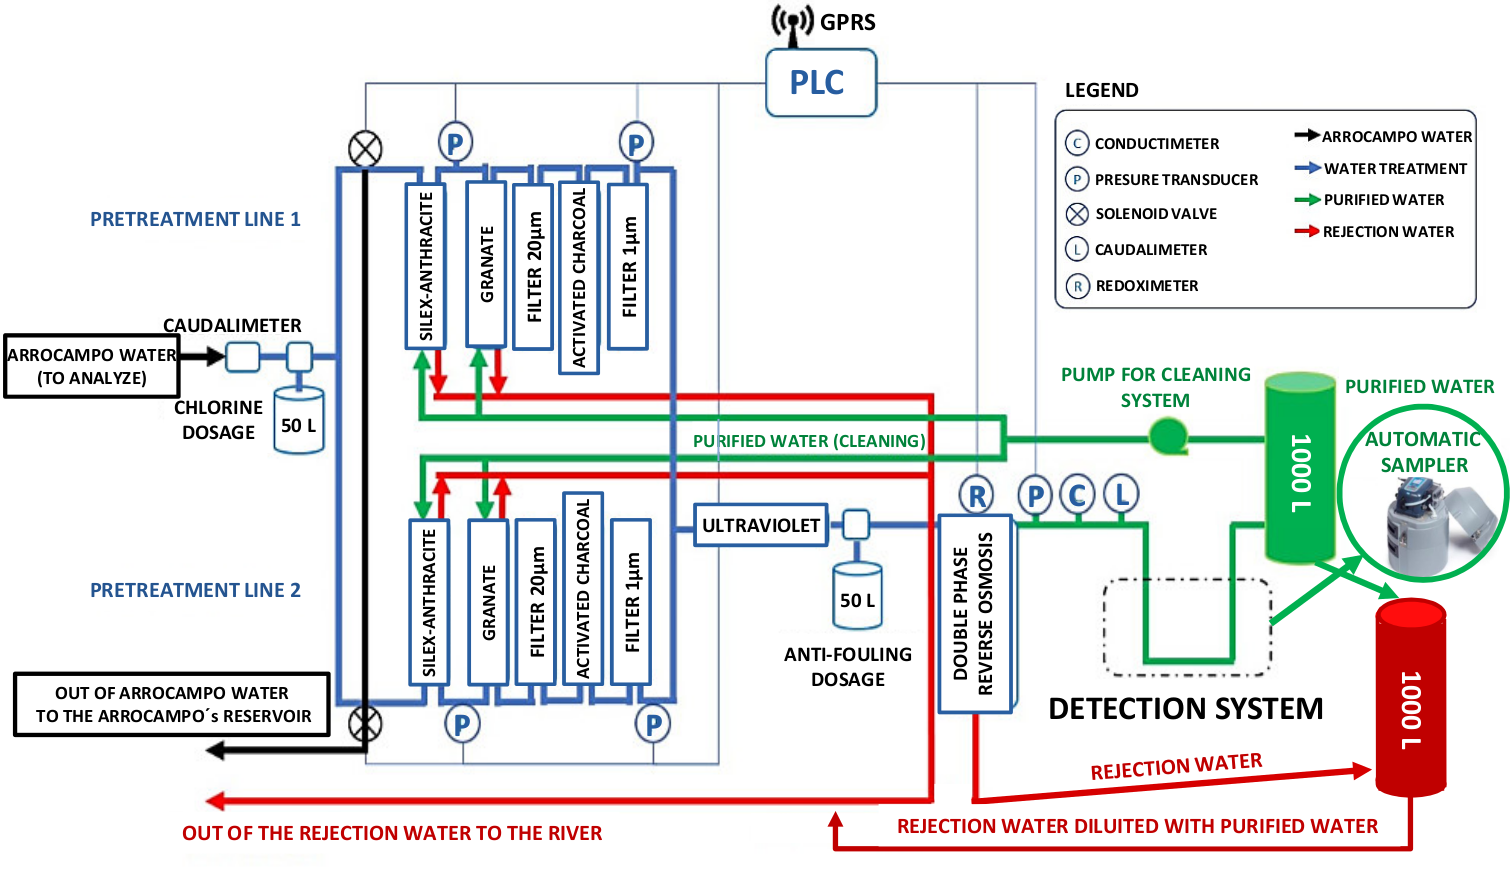
\includegraphics[scale=0.25]{3DesignPrinciples/33UltraPureWaterSystem/SchemeUltraPureWaterSystem.png}
\caption{Scheme of water purification system.\label{fig:WPSScheme}}
\end{figure}

This system has been installed in the Arrocampo dam and consists of four different consecutive stages:

\begin{itemize}
\item{} First, the raw water from the Tagus River is introduced into two different filters, the first formed by Silex-Anthracite and the second by granate, with which we make a gross filtering (the largest particles are eliminated). There are two parallel lines that are capable of self-cleaning by injecting ultrapure water in the opposite direction.

\item{} Next, this water sample is introduced into a $20~\mu\meter$ filter (Formed by a synthetic mesh) and activated charcoal filters (one per line in both) that form the fine filtration stage. With the $20~\mu\meter$ filter we can filter particles with diameters of up to $20\mu\meter$ and, with the activated charcoal filter, we remove the chlorine and iron particles from the sample.

\item{} Then, this water sample is introduced into the super-fine filtering consisting of a $1~\mu\meter$ filter, formed of a dense polypropylene mesh, (one per line), and UV lamps. With the first we remove all the particles up to diameters of $1~\mu\meter$ and, with the second, we remove the organic matter present in the purified water sample.

\item{} Finally, this water sample is introduced in the last stage, double-phase reverse osmosis, thereby reducing the conductivity of the water to values of $5~\mu$S$/\cm$. We verified that we achieve a conductivity of $10~\mu$S$/\cm$ with only one module reverse osmosis and this is enough for the needed conditions of tritium detector. Therefore, we use just one module of reverse osmosis for $24~\hour$ and the other for another $24~\hour$, thereby reducing the power consumption of the system.

\end{itemize}

At the end of this system, each water sample is divided into two different outlet samples. The pure water sample, which is the ultrapure water that will be injected into tritium detector, and the rejection water, whose turbidity is even greater than the water sample before treatment because it contains all the particles that have been extracted from the ultrapure water sample.

With this ultrapure water system we can process up to $0.850~\meter^3/\hour$ with a single line operating or $1.480~\meter^3/\hour$ with both, greatly overestimating the requirements of the tritium detector. 

The software used for remote controlling the ultrapure water system is Siemens PLC, with which we receive information fo this system sush as the state of the valves, the pressure probes or water production in real time. 

In the appendix \ref{App:UltraPureWaterSystem} there are several photos showing each part of this system.